In order to produce enough musical examples and references for a student to use, some automated way of producing the referential manuscript is ideally needed and several tools exist to help with this. Each is designed to cater to slightly different needs but all of the below merit at least brief mentions.

\subsection*{Professional GUI Tools}
\label{sec:ProfTools}
There are several professional tools which are used in industry to generate musical scores on the computer. The ones with most widespread usage are Sibelius\footnote{http://www.avid.com/US/products/SibeliusFirst/overview} and Finale\footnote{http://www.finalemusic.com/products/finale/} and more recently, NoteFlight\footnote{http://www.noteflight.com/}

They're worth mentioning as they're the ``industry standards'' for musical notation and composition, used by professionals and in education around the world, but their primary use case is manual input via a GUI so for our purposes they are not ideal.

\subsection*{LilyPond}
\label{sec:lilypond}

LilyPond\footnote{http://www.lilypond.org/} is a music engraver and serves as a \enquote{modular, extensible and programmable compiler for producing high-quality music notation}. Originally inspired by the efforts of projects like MusixTex\footnote{http://www.mab.jpn.org/musictex/musixtex\_e.html} which had aimed to \enquote{be able to typeset complex polyphonic, orchestral or instrumental music}\cite{Taupin99musixtex–using} in the same way that it was already renowned for beautifully typeset text and maths. It's a widely adopted tool but it's flexibility with regard to formatting made it difficult to learn.

The idea of Lilypond was that by entering or programmatically generating a formal representation of music which is designed to be easy to type, you can then use LilyPond to produce a manuscript engraving form that representation. They also support conversion from other popular text-based music formats such as MusicXML\footnote{Some good examples can be found at http://www.musicxml.com/tutorial/hello-world/}, or ABC\footnote{Standards can be found at http://abcnotation.com/}.

For example, given the following LilyPond syntax:

\begin{lstlisting}
\relative c' {
  c' d' e' f' g'2 g'2
}
\end{lstlisting}

We can run LilyPond to produce the following output:

\begin{lilypond}[fragment, staffsize=26]
  c' d' e' f' g'2 g'2
\end{lilypond}

Using Lilypond and some basic algorithms around music theory we could happily generate textual representations of exercises and generate the necessary images from them. It's also free and accessible meaning that I can easily install it on development machines and servers. Indeed, Lilypond is the primary method by which I have generated the manuscript examples in this dissertation.

\subsection*{VexFlow}

Vexflow\footnote{https://github.com/0xfe/vexflow} is another music engraving application, but Vexflow is web based and uses HTML5 Canvas\footnote{https://developer.mozilla.org/en/docs/HTML/Canvas} and SVG\footnote{http://en.wikipedia.org/wiki/Scalable\_Vector\_Graphics}. As such it can be used to generate manuscripts on the fly in a browser. The limitations of alternate solutions such as \nameref{sec:lilypond} are that for use on the web, they need to render the music remotely on the server, then synchronously or asynchronously transport those resources (most likely images which are expensive for web traffic) to the client.

One key feature Vexflow has over local software like Lilypond is that since it utilises canvas elements it also allows programmatic real-time manipulation of the rendered score.

For example if you were to include the vexflow library and then write the following javascript:

\begin{lstlisting}[language=JavaScript]
var canvas = $("div.one div.a canvas")[0];
var renderer = new Vex.Flow.Renderer(canvas,
  Vex.Flow.Renderer.Backends.CANVAS);

var ctx = renderer.getContext();
var stave = new Vex.Flow.Stave(10, 0, 500);
stave.addClef("treble").setContext(ctx).draw();
\end{lstlisting}

Vexflow would render the following:


\begin{figure}[h!]
  \frame{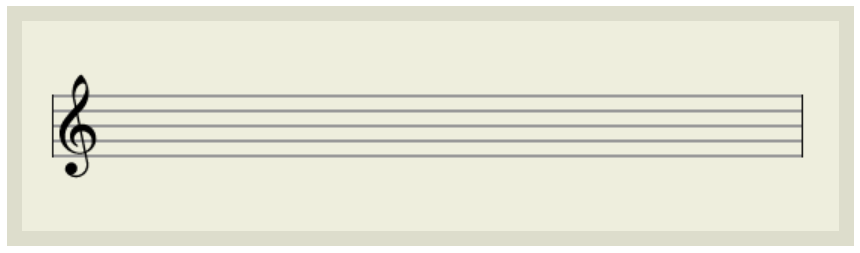
\includegraphics[width=\linewidth]{gfx/vexflow.png}}
  \centering
  \caption{Vexflow render, see \url{http://vexflow.com/docs/tutorial.html}}
  \label{fig:VexflowOutput}
\end{figure}

Vexflow is open source and currently under active development.

